\FloatBarrier
\section{Behavioral Cloning}
\label{sec::71_bc}
The first approach to train a neural network on autonomous navigation is based upon behavioral cloning. The generation concept will be explained in section \ref{sec::711_gc}, while implementation details will be provided in the subsequent section \ref{sec::712_id}.
\FloatBarrier
\subsection{General Concept}
\label{sec::711_gc}
Behavioral cloning in itself is not always related to machine learning but poses one possible way of training a neural network in a supervised manner. The presented concept is easy to understand and got inspired by \cite{bojarski2016end}, where it was used for self-driving cars. It utilizes the control loop, which was already introduced in figure \ref{fig::7_cl}. In order to then replace the human user by an artificial agent, one has a human user perform a desired behavior, and copy it. The required extended control loop is shown in figure \ref{fig::71_bc}.
\begin{figure}[h!]
	\centering
	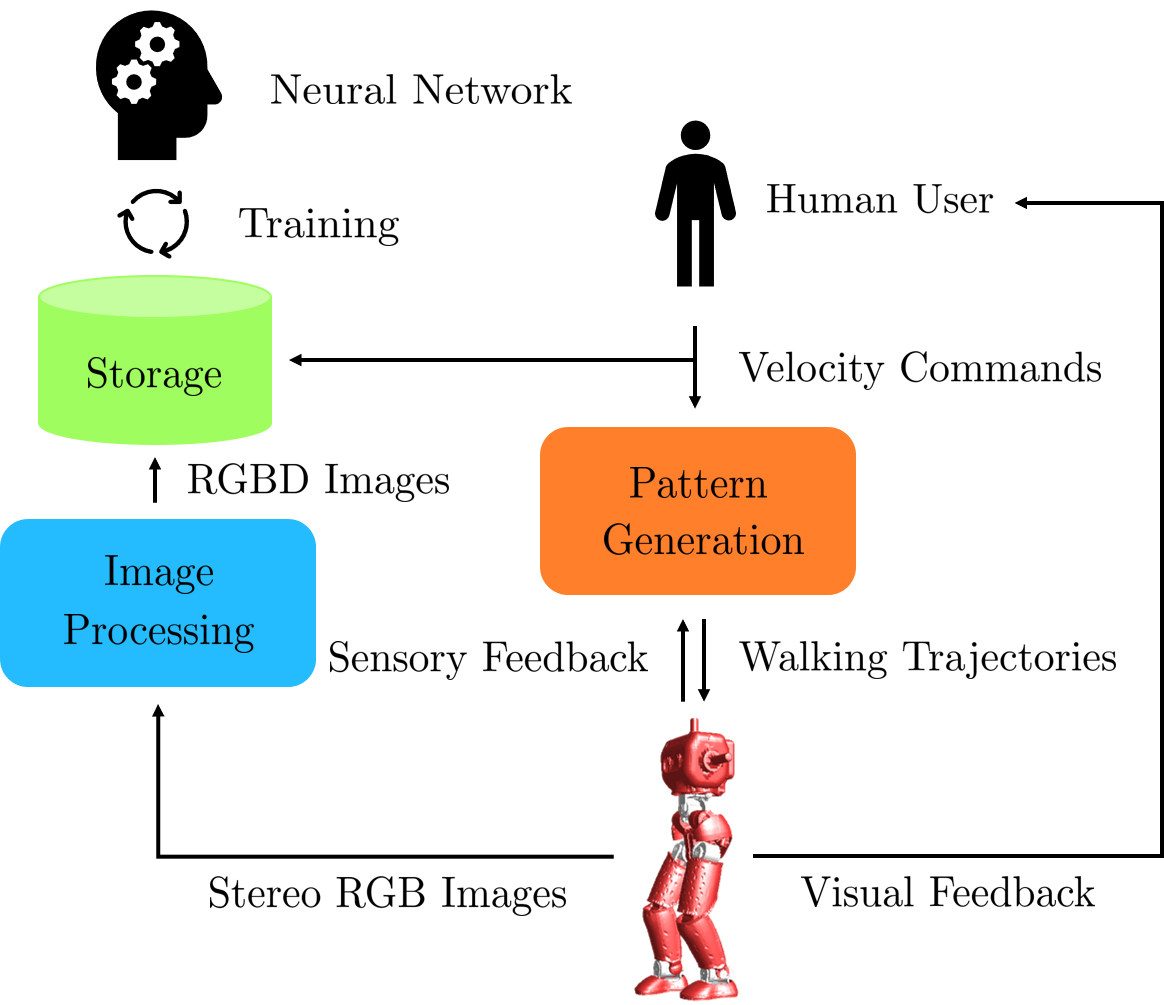
\includegraphics[scale=.5]{chapters/07_autonomous_high_level_control_of_the_walking_pattern_generator/img/behavioral_cloning.png}
	\caption{Pipeline for behavioral cloning. The neural network is trained on stored RGBD images, and corresponding velocity commands that are correlated by a timestamp.}
	\label{fig::71_bc}
\end{figure}
It takes the velocity commands from the human user and stores them alongside images with a corresponding timestamp to a storage. The timestamp allows to correlate seen images to desired velocities afterward, which in turn enables an artificial agent to train on the stored data. Within this thesis, the artificial agent is a neural network. An appropriately chosen network architecture will then enable one to learn the taught behavior, and it ultimately allows to replace the human user. This procedure relies on prior knowledge to achieve certain tasks, namely the stored data. It is therefore essential to assure that the sampled data, from which a task is learned, does not introduce any unwanted bias. That is, one needs to take care of the distribution from which one samples in the first place. In principle, it is possible to learn any arbitrary behavior with this technique, but this requires not only good data, but also a vast amount of it, which may not always be available. However, there exist domains from which it is undeniably easier to learn a task. To equip a neural network with some prior knowledge by switching the domain may therefore not only be highly desirable but sometimes also needed if the amount or quality of data is not sufficient. One domain which is of special interest when it comes to interacting in a three-dimensional environment is a domain that represents depth information. If there are any, it may sometimes be possible to extract this kind of prior knowledge from a depth camera. However, Heicub does not support RGBD cameras, but only stereo RGB cameras. An additional image processing step is therefore introduced to the proposed pipeline, as indicated by the blue box in figure \ref{fig::71_bc}, which extracts RGBD images from stereo RGB images. Implementation details, are given in the following section.
\FloatBarrier
\subsection{Implementation Details}
\label{sec::712_id}
Heicub does only support a pair of stereo RGB cameras, and the RGBD images are, therefore, obtained via weighted least squares disparity maps, which got explained in section \ref{sec::3_ip}. This extraction of the depth information is part of the image processing block of figure \ref{fig::71_bc}, and it relies on OpenCV \cite{opencv_library}, just as the stereo camera calibration does, which is a requirement for the computation of depth maps via stereo block matching algorithms. The recorded RGBD images, and the corresponding velocities are stored inside of a folder. Locations to the image files, as well as the velocities, are then saved to a text file. This procedure allows to train a neural network on the database. As the pattern generation library is written in C++ for efficiency, but further for compatibility with Heicub's communication system, so has the neural network. However, the deep learning training pipeline is implemented within Python using PyTorch \cite{paszke2017automatic} to allow for a faster prototyping, for which the routine can be found at the provided \href{https://github.com/mhubii/nmpc_pattern_generator/blob/master/libs/learning/python/train_rgbd.py}{\underline{link}}. This pipeline mainly implements a \inlinecode{}{torch.utils.data.Dataset}, which loads the RGBD images with their corresponding velocity labels to a \inlinecode{}{torch.tensor}. Moreover, the implemented dataset performs pre-processing steps, which include image cropping, normalization, and reshaping. A neural network model that is trained in this way, can then be converted to a just in time (JIT) script that can be loaded into C++ via
\begin{minted}{cpp}
  auto module = torch::jit::load(net_location);
\end{minted}
The code to convert a model, can be found at the following \href{https://github.com/mhubii/nmpc_pattern_generator/blob/master/libs/learning/python/python_to_cpp.py}{\underline{link}}. Once the neural network is trained to predict a desired velocity for the pattern generation, one only has to convert the desired velocity from a \inlinecode{}{torch::Tensor} to an \inlinecode{C++}{Eigen::Vector3d}, which is the datatype that the pattern generation library works with. This velocity is then forwarded, via the \inlinecode{}{NMPCGenerator::SetVelocityReference} method, just as described in section \ref{sec::63_us}, and a new iteration is executed.